\begin{center}
    \large \textbf{3. Előadás}\\
    Merev test kinematikája
\end{center}
\setstretch{1.5}
\textbf{Elméleti összefoglaló:}\\
\textbf{A merevtest síkmozgás kinematikája:}\\
Az eddig bevezett összefüggések merevtestek tetszőleges térbeli mozgására vonatkoztak. Fontos speciális eset az, amikor a merevtest síkmozgást végez, ekkor ugyanis egyszerűbb alakra hozható mind a sebességredukciós mind a gyorsulásredukciós képlet.\\
A test pontjai egymással párhuzamos síkokban mozognak és minden pont sebesség és gyorsulásvektora is párhuzamos ezekkel a síkokkal. Ekkor a szögsebességvektornak merőlegesnek kell lennie a mozgás síkjára.\\
Míg az általános esetben a sebesség- és gyorsulásállapot együttes megadásához 12 skalár komponenst kell megadni, síkmozgás esetén mindössze hat nem zérus komponens marad.
\begin{multicols}{4}
    $$\underline{v}_A = 
    \begin{bmatrix}
        V_{Ax} \\
        V_{Ay} \\
        0
    \end{bmatrix}
    $$

   \columnbreak

   $$\underline{a}_A = 
    \begin{bmatrix}
        a_{Ax} \\
        a_{Ay} \\
        0
    \end{bmatrix}
    $$

    \columnbreak

    $$\underline{\omega}_A = 
    \begin{bmatrix}
        0 \\
        0 \\
        \omega_z
    \end{bmatrix}
    $$

    \columnbreak

    $$\underline{\varepsilon }_A = 
    \begin{bmatrix}
        0 \\
        0 \\
        \varepsilon_z
    \end{bmatrix}
    $$


    
\end{multicols}
\textbf{Megjegyzés:} \(\varepsilon\) előjelet a tangenciálus gyorsulás előjeléhez megfelelően kell értelmezni. Akkor pozitív, ha a szögsebesség abszolút értéke nő. Ha \(\underline{\varepsilon} = \underline{0} \Rightarrow \underline{\omega} = \) állandó
\begin{tcolorbox}[colback=MidnightBlue!5!white,colframe=MidnightBlue!60!black,title= Definíció]
   Álló tengely körüli forgás esetén az \(\alpha\) gyorsulászög a gyorsulásvektortól a normális gyorsulásvektor irányáig felmért előjeles szög:
   $$\tan(\alpha) = \dfrac{\varepsilon_z}{\omega^2}$$
\end{tcolorbox}
\textbf{Síkmozgást végző merevtest sebességállapota:}\\
A síkmozgást végző testek csak haladó vagy forgó mozgást végezhetnek, csavarmozgást nem. \\
Általános síkbeli forgó mozgást végző merev test esetén akkor egyszerűsödnek le a sebességállapotra vonatkozó egyenletek, ha a pillanyatni forgástengely \(xy\) síkba eső \(P\) pontját választjuk referenciapontnak. A nulla sebességű pontot sebességpólusnak nevezzük.
\begin{tcolorbox}[colback=MidnightBlue!5!white,colframe=MidnightBlue!60!black,title= Definíció]
    Síkmozgást végző merev test nulla sebességű \(P\) pontját póluspontnak vagy sebességpólusnak nevezzük.
    A \(P\) sebességpólusnak ismeretében egy tetszőleges \(B\) pont sebessége felírható:
    $$\underline{v}_B = \underline{v}_p + \omega \times \underline{r}_{PB} = \omega \times \underline{r}_{PB}$$
    kihasználva a síkmozgás sajátosságait
    \begin{center}
    \(v_B = \omega \mid \underline{r}_{PB} \mid\) és \(\underline{v}_b \perp \underline{r}_{PB}\)
    \end{center}
    A sebesség nagysága arányos a sebességpólustól mert távolsággal, iránya pedig merőleges a sebességpólusból húzott helyvektora. A síkmozgást végző test a sebességállapota szempontjából úgy viselkedik, mintha a \(P\) sebességpólus körül forogna.
 \end{tcolorbox}
 \textbf{A sebességpólus meghatározása:}
 \begin{itemize}
    \item sebességredukciós képletből
    \item szerkesztéssel
    \item \(\underline{r}_{AP} = \dfrac{\underline{\omega} \times \underline{v}_A}{\omega^2}\) (A pontból, centrális egyenes...)
 \end{itemize}
 Következik, hogy \(\underline{v}_A \perp \underline{r}_{AP}\). Ez lehetőséget ad a sebességpólus helyének gyors geometriai meghatározására: két ponz sebességvektorára merőlegeseket állítva a kapott egyenesek kimetszik a sebességpólus helyét.\\
 Az ismertetett eljárás síkbeli haladó mozgásra is általánosítható. Egy haladó mozgást végző test sebességpólusa a sebességvektorra merőleges irányban egy végtelen távoli pontban képzelhető el.
 \\
 \textbf{Síkmozgást végző merevtest gyorsulásállapota:}
 \begin{tcolorbox}[colback=MidnightBlue!5!white,colframe=MidnightBlue!60!black,title= Tétel]
    Síkmozgás esetén a gyosulásredukciós képlet egyszerűsödik
    $$\underline{a}_B = \underline{a}_A + \varepsilon \times \underline{r}_{AB} - \omega^2 \underline{r}_{AB}$$
 \end{tcolorbox}
 Az általános síkmozgást végző merevtest vissazvezethető álló tengely körüli forgásra, ha a testnek van egy kiválasztott nulla gyorsulású pontja. Ez a pont általában nem esik egybe a sebességpólussal, mivel a \(P\) sebességpólus helye független a gyorsulásállapottól, annak gyorsulásra általában nem nulla.
 \begin{tcolorbox}[colback=MidnightBlue!5!white,colframe=MidnightBlue!60!black,title= Definíció]
    A gyorsulás helye
    $$\underline{r}_{AB} = \dfrac{\omega^2\underline{a}_A + \varepsilon \times \underline{a}_A}{\varepsilon^2 + \omega^4}$$
    képlettel adható meg.
 \end{tcolorbox}
Ha egyszerre \(\varepsilon = 0, \omega = 0\) és \(\underline{a}_A = 0\), akkor nem értelmezhető a képlet, mert a test minden pontja nulla gyorsulású. Ha \(\varepsilon =0, \omega = 0\) és \(\underline{a}_A \neq 0\), akkor haladó mozgást végez a test, ezért gyorsuláspólusa a végtelenbe kerül.\\
A gyorsulás nagysága:
$$a_A = \mid \underline{r}_{GA} \mid \sqrt{\varepsilon^2 + \omega^4}$$
azaz arányos a gyorsuláspólustól mért távolsággal, ugyanúgy, mint álló tengely körüli forgásnál. Tehát a síkmozgást végző merev testnek az a pontja mozog legnagyobb gyorsulással, amelyik legmesszebb van a gyorsuláspólustól.
\begin{tcolorbox}[colback=MidnightBlue!5!white,colframe=MidnightBlue!60!black,title= Definíció]
    Általános síkmozgás esetén a gyorsulásredukciós képletben szereplő \((\omega^2 \underline{r}_{GA})\) vektor az \(A\) pontból a \(G\) gyorsuláspólus felé mutat és definíció szerint \(\alpha \) gyorsulászöget zár az \(A\) pont gyorsulásvektorával. A gyorsulászög független az \(A\) pont választásától. Előjelet a szöggyorsulás iránya határozza meg:
    $$\tan(\alpha) = \dfrac{\varepsilon_z}{\omega_z}$$
\end{tcolorbox}
\textbf{Megjegyzés:} \(\varepsilon\) irányában \(\alpha\) szöggel elforgatott egyeneseket mérünk fel, ezek kimetszik a gyorsuláspólust.
 \textbf{Sebességpólus, gyorsuláspólus és a pálya görbületi közzéppontja:}\\
 Úgy tekinthetjük mintha a sebességek szempontjából a \(P\) sebességpólus körül, a gyorsulások szempontjából pedig a \(G\) gyorsuláspólus körül forogna a test.  Ugyanakkor a merevtest pontjainak pályái különbözőek és a pályák egyes pontjaihoz is más és más görbületi középpont tartozik, a merevtestnek egy adott időpillanatban csak  egyetlen \(P\) sebességpólusa és egyetlen \(G\) gyorsuláspólusa van. 
 A görbületi közppont helye csak a kiválasztott pont pályától függ. Ezzel szembena sebességpólus helyét csak a sebességállapot, a gyorsuláspólus heéyét pedig csak a gyorsulásállapot határozza meg. Ezért ezek a pontok általában nem esnek egybe csak álló tengely körüli forgás esetén.\\
\newpage
 \textbf{A gördülés kinematikája:}\\
Síkmozgás során általában változik a sebességpólus helye a mozgés során. Például ha kerék átmegy egy víztócsán, a testen és a talajon a nedves pontok jelölik ki azokat a görbéket, melyek pontjai valamikor póluspontok voltak. \\
A merevtest pontjainak sem a sebessége, sem a szögsebessége nem változhat ugrásszerűen, ezért a pillanatnyi forgástengely és a sebességpólus helye folytonosan változik. Mivel a gördülő test és a telej pontjai az érintkezés után eltávolodnak egymástól, két görbét is definiálhatunk, melynek pontjai póluspontok voltak, illetve lesznek: egy gördülő kerék esetében a kerék által a talajon hagyott nyom jelölik ki az álló pólusgörbét, a kerék azon pontjai pedig, melyek póluspontok voltak, a mozgó pólusgörbén helyezkednek el.
\begin{tcolorbox}[colback=MidnightBlue!5!white,colframe=MidnightBlue!60!black,title= Definíció]
    Az álló pólusgörbe a \(P\) sebességpólus, mint geometriai pont pályája a vonatkoztatási rendszerben.
 \end{tcolorbox}
\begin{tcolorbox}[colback=MidnightBlue!5!white,colframe=MidnightBlue!60!black,title= Definíció]
    Az álló pólusgörbe a \(P\) sebességpólus, mint geometriai pont pályája a merevtesthez képest.
 \end{tcolorbox}
 Gördülés soran a nulla sebességű sebességpólus változtatja helyét a síkban, ezt a folyamatot pólusvándorlásnak nevezzük.
\begin{tcolorbox}[colback=MidnightBlue!5!white,colframe=MidnightBlue!60!black,title= Definíció]
    A pólusvándorlás sebessége a \(P\) sebességpólus, mint geometriai pont sebessége, ahogy halad az álló pólusgörbén, jele: \(\underline{U}\)
    \begin{center}
        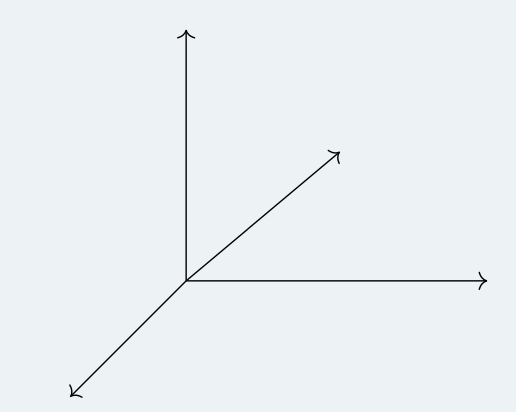
\includegraphics[scale = 0.7]{Ea_gyak_1/2.png}
    \end{center}
    Az \(\underline{u}\) pálusvándorlási sebességnek gyakran ismert az iránya, hiszen ha egy test egy másikon gördül, akkor a közös érintővel párhuzamosnak kell lennie.
\end{tcolorbox}

\textbf{Megjegyzés:}\\
Minden, nem nulla szögsebességű síkmozgást végző merevtest mozgása értelmezhető a mozgó pólusgörbének az álló pólusgörbén történő gördülésként, ahol az aktuális érintkezési pont a \(P\) póluspont.

\begin{tcolorbox}[colback=MidnightBlue!5!white,colframe=MidnightBlue!60!black,title= Tétel]
A pólusvándorlés \(\underline{u}\) sebessége \(\underline{u} = \dfrac{\underline{\omega} \times \underline{a}_p}{\omega^2}\), ahol \(\underline{a}_p\) a sebességpólus gyorsulásra. Valamint
\begin{center}
    \(\underline{u} \perp \underline{\omega}\) és \(\underline{u} \perp \underline{a}_p\)
\end{center}
\end{tcolorbox}



\newpage
\begin{center}
    \large \textbf{3. Gyakorlat}\\
    Gördülő korong, bolygómű
\end{center}
\begin{tcolorbox}[colback=MidnightBlue!5!white,colframe=MidnightBlue!60!black,title= 1. Feladat{,} egyenes kényszerpályán gördülő korong]
    \setstretch{1.2}
        \textbf{Adatok:}
    \begin{center}
        \begin{multicols}{3}
            \(v_s = 1\ ms^{-1}\)
    
            \columnbreak
    
            \(a_s = 2\ ms^{-2}\)
    
            \columnbreak
    
            \(r = 0,5\ m\)
        \end{multicols}
    \end{center}
    \textbf{Feladatok:}
    \begin{itemize}
        \item Síkban gyorsulva gördülő korongról melyik pontban válnak le a legkönnyebben a sárcseppek azaz \(a_{max} = a_q ;\hspace{10pt} \underline{r}_{sq} = ?\)\\
        \\
        \textbf{Részfeladatok:}
        \begin{itemize}
            \item \(\underline{\omega} = ?\), sebességpólus helye \(\underline{r}_{sp} = ?\)
            \item \(\underline{\varepsilon} = ?\), gyorsuláspólus helye \(\underline{r}_{ss} = ?\)
            \item sebességpólus gyorsulása, \(\underline{a}_p = ?\)
            \item gyorsuláspólus sebessége, \(\underline{v}_G =?\)
        \end{itemize}
    \end{itemize}
    \Pointilles{20}
\end{tcolorbox}
\begin{tcolorbox}[colback=MidnightBlue!5!white,colframe=MidnightBlue!60!black,title= 2. Feladat{,} hajtómű sebesség és gyorsulásállapot]
    \setstretch{1.2}
        \textbf{Adatok:}
    \begin{center}
        \begin{multicols}{3}
            \(\omega_1 = 10\ rads^{-1}\)
    
            \columnbreak
    
            \(\varepsilon = 5\ rads^{-2}\)
    
            \columnbreak
    
            \(r = 0,1\ m\)
        \end{multicols}
    \end{center}
    \textbf{Feladatok:}\\
    \textbf{I. Sebességállapot}
    \begin{itemize}
        \item Számítsa ki a (3) kerék szögsebességét és súlypontjának sebességét \(\underline{\omega}_3 = ?, \underline{v}_{s3} = ?\)
        \item Mekkora szögsebességgel kering a (3)-as test súlypontja \((\underline{\omega}_2 = ?)\)
        \item Rajzolja meg a sebességeloszlást az \(\overline{AB} \) szakaszon!
    \end{itemize}
    \textbf{II. Gyorsulásállapot}
    \begin{itemize}
        \item Számítsa ki a (3) kerék súlypontjának gyorsulását \((\underline{a}_{s3} = ?)\)
        \item Határozza meg az \(A\) és \(B\) pontok gyorsulásait: \((\underline{a}_A, \underline{a}_{B1}, \underline{a}_{B3}) = ?\)
        \item Határozza meg a (3) kerék gyorsuláspólusának helyét!
        \item Rajzolja meg a gyorsulásábrát!
    \end{itemize}

    \Pointilles{20}
\end{tcolorbox}